\documentclass[pageno]{jpaper}

%replace XXX with the submission number you are given from the ASPLOS submission site.
\newcommand{\asplossubmissionnumber}{127}

\usepackage{times}
\usepackage{datetime}
\usepackage{balance}  % to better equalize the last page
\usepackage{graphics} % for EPS, load graphicx instead
\usepackage{url}
\usepackage{hyperref}
\usepackage{txfonts}
\usepackage{pslatex}    
\usepackage{pifont}
%\usepackage{bbding}
\usepackage{multirow}
\usepackage{makecell}
\usepackage[justification=centering]{caption}
\usepackage{xspace}
\usepackage{comment}
\usepackage{listings}
%\usepackage[section]{placeins}
\usepackage{tikz}
\usepackage{calc}
\usepackage{fancyvrb}
\usepackage{xcolor}
\usepackage{flushend}
\usepackage{wrapfig}

\newcommand{\cmark}{\ding{51}}%
\newcommand{\xmark}{\ding{55}}%

\newcommand{\eurosyssubmissionnumber}{\#147, 12 pages}
\newcommand{\todo}[1]{{\color{red}\bfseries [[#1]]}}
\newcommand{\TP}[1]{{\color{red}\bfseries [[#1]]}}

\newcommand{\specialcell}[2][c]{%
  \begin{tabular}[#1]{@{}c@{}}#2\end{tabular}}
\newcommand{\OB}{\texttt{OpenBSD}}
\newcommand{\DieHarder}{\texttt{DieHarder}}
\newcommand{\DL}{\texttt{DLmalloc}}
\newcommand{\JE}{\texttt{jemalloc}}
\newcommand{\MP}{\texttt{mmprof}}
\newcommand{\RN}[1]{\uppercase\expandafter{\romannumeral #1\relax}}


\begin{document}

\title{mmprof: A General Profiler for Different Memory Allocators\\ \textbf{Extended Abstract}}

\date{}

\maketitle

% No abstract needed for the extended abstract
%\begin{abstract}
%\end{abstract}


\section{Motivation}
\label{sec:motivation}

A memory allocator is a key component that could significantly impact the performance and memory consumption of the corresponding applications by up to orders of magnitude. However, none of existing tools could answer the following questions related to the memory allocator. \\

\begin{itemize}
\item \textbf{Q1:} \textit{Whether the allocator introduces some performance slowdown for this application? }
\item \textbf{Q2:} \textit{How much the performance can be improved if switching to a well-performed allocator (e.g., TcMalloc)?}
\item \textbf{Q3:} \textit{How much memory wastes the allocator introduces?}
\item \textbf{Q4:} \textit{What are the possible design issues for performance slowdown?}
\item \textbf{Q5:} \textit{What are the reasons for memory wastes?} 
%\item What are quantitative metrics to evaluate a memory allocator? 
\end{itemize}
\vspace{0.1in}

Due to the obvious importance of a memory allocator, it is emergent to design a profiler that could answer these research questions about an allocator. This paper presents such a profiler--\MP{}--that profiles different aspects of an allocator, which will benefit both allocator designers and normal users. 

\MP{} will benefit normal users by predicting potential performance impact, reporting detailed memory wastes, and judging whether an allocator is tapped with allocation/deallocation pattern or access pattern of the current application. \MP{} will also benefit allocator designers that help diagnose the specific design issues inside the allocator. 

\section{Limitations of the State of the Art}
\label{sec:limitations}

None of existing profilers can identify the inherent reasons of performance slowdown and memory wastes caused by an allocator. 

General profilers, such as \texttt{gprof}~\cite{DBLP:conf/sigplan/GrahamKM82} and \texttt{perf}~\cite{perf}, only report the time accumulation of different functions, and \texttt{Coz}~\cite{Coz} presents a quantitative performance impact of improving a particular region of code. Although they may identify some performance bottlenecks inside applications, but they could not shed light on the performance issues caused by the allocator. 

 Existing allocator profilers, such as \texttt{mprof}~\cite{Zorn:1988:MAP:894814}, Mtrace~\cite{mtrace}, Mtrace++~\cite{Lee:2000:DMM:786772.787150}, \texttt{TcMalloc} profiler~\cite{tcmalloc-profiler}, or CLR profiler~\cite{lupasc2014dynamic}, mainly focus on how an application uses the memory, but not on memory wastes caused by the allocator itself. 


\section{Key Insights}
\label{sec:key-insights}

%\begin{itemize}
%\item What are the one or two key new insights in this paper?
%\end{itemize}

\MP{} aims to identify the performance and memory impact caused by the allocator. However, the key question is that what aspects of an allocator could introduce the performance and memory impact? 

Based on our observation, an allocator can affect the performance of applications in two ways: first, the performance of memory management operations will affect the performance of applications, where slow operations may degrade the performance.  Second, whether an allocator is tapping well with memory usage and access pattern of a particular application, called ``\textit{application friendliness}'', including cache utilization rate, page utilization rate, passive/active false sharing, and cache invalidation rate. 

The performance of memory management operations can be affected by the following factors. The first reason is due to the complexity of the implementation, which can be measured by the number of instructions inside each operation. The second reason can be caused by some hardware events of the algorithm design, such as cache misses. The third reason can be caused by user space contention, which could be evaluated via lock acquisitions and lock contention inside each memory management operation. The fourth reason is due to kernel contention, which could be caused by memory-related system calls. Based on this observation, \MP{} proposes to utilize hardware Performance Monitoring Units (PMUs) to collect the number of instructions and hardware events inside each memory operation, and intercepts synchronizations and memory related system calls in order to identify user and kernel space contention. It further utilizes RTDSC timestamp to measure the runtime. The basic idea is shown as Figure~\ref{fig:basicidea}. 

\begin{figure}[!ht]
\centering
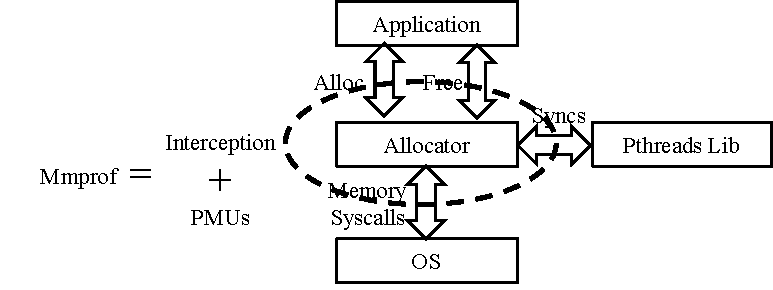
\includegraphics[width=3in]{figures/basicidea}
\caption{Basic idea of \texttt{mmprof}.\label{fig:basicidea}}
\end{figure}


\MP{} reports different types of memory wastes introduced by an allocator. Based on our observation, memory wastes of an allocator can be caused by the following aspects: metadata overhead, internal fragmentation, memory blowup, and external fragmentation.  Although it is straightforward to measure internal fragmentation, but not for memory blowup and external fragmentation. Memory blowup occurs when memory deallocations from one thread cannot be utilized to satisfy subsequent memory requests from other threads~\cite{Hoard}, due to the employment of per-thread heaps. However, this definition cannot be utilized directly to collect the total memory blowup, as it does not specify how to update it upon consequent deallocations and re-allocations. \MP{} measures memory blowup with a key observation: \textit{the total size of freed objects represent the upper bound of memory blowup for a size class}. Then the memory blowup can be measured by subtracting the total size with the size of recently-freed objects. After computing the memory blowup, \MP{} is able to compute the overhead of external fragmentation and metadata afterwards. 
 



%\begin{itemize}
%\item What makes it more effective than past approaches?
%\end{itemize}


\section{Main Artifacts}
\label{sec:main-artifacts}

%\begin{itemize}
%\item What are the key artifacts presented in your paper: a methodology, a hardware design, a software algorithm, an optimization or control technique, etc.?
%\end{itemize}

The key artifacts is a profiling tool that could identify different aspects of an allocator, such as performance, memory, application-friendliness. 

\MP{} is designed as a drop-in library that can be simply linked to applications (and allocators) with the preloading mechanism, which does not require the change or the re-compilation of applications and allocators, as far as an allocator utilizes standard synchronizations and system calls.

We evaluated \MP{} with five widely-used allocators, including two versions of the Linux allocator (versions 2.21 and 2.28), TCMalloc~\cite{tcmalloc}, jemalloc, and Hoard, and one secure allocator--DieHarder. Overall, the evaluation includes the effectiveness and the overhead. The experimental results show that \MP{} successfully identifies multiple known and \textbf{unknown} design issues inside popular allocators. Due to its careful design, \MP{} only imposes 35\% performance overhead on average. This efficient design reduces \MP{}'s interference to the original execution. \MP{} does not need the change of the allocator, the application, and the underlying OS, which will be convenient for the employment. 


%\MP{} is the first systematic approach to evaluate and profile different memory allocators, without changing the internal implementation of allocators. More specifically, \MP{} proposes the combination of function interception (based on common APIs) and PMU-based sampling to perform the profiling. Besides, \MP{} proposes the first tool to quantitatively measure memory blowup (and external fragmentation), cache/page utilization rate, and passive/active false sharing impact.  

%\begin{itemize}
%  \item How were your artifacts implemented and evaluated? 
%\end{itemize}

\noindent
\MP{} is written as a runtime library that could be attached to different allocators, as far as . 

\section{Key Results and Contributions}
\label{sec:key-contributions}

\begin{comment}

\begin{itemize}
  \item What are the most important \emph{one or two} empirical or theoretical
    results of this approach?
\end{itemize}

\begin{itemize}
  \item What are the contributions that this paper makes to the state of the
    art? List them in an \texttt{itemize} section. Each contribution should be no more than a few sentences long.
\end{itemize}

\begin{itemize}
  \item Clearly describe its advantages over past work, including how it overcomes their limitations.
\end{itemize}
	
\end{comment}

This paper makes the following contributions. 

\begin{itemize}
\item \MP{} is the first systematic approach to evaluate and profile different memory allocators, without changing the internal implementation of allocators. More specifically, \MP{} proposes the combination of function interception (based on common APIs) and PMU-based sampling to perform the profiling.
 

\item \MP{} analyzes multiple relevant factors that an allocator may impact the performance of applications.


\item \MP{} proposes the first experimental mechanisms to quantitatively measure memory blowup (and external fragmentation), cache/page utilization rate, and passive/active false sharing impact. 

\item This paper performs extensive experimentation to confirm \MP{}'s effectiveness and overhead. The experiments also uncovers multiple known and unknown design issues in widely-used allocators.  

\end{itemize} 


\section{Why ASPLOS}
\label{sec:why-asplos}

This paper describes a tool that could be utilized to identify performance and memory issues brought by the memory allocator. Since the tool belongs to the runtime system, it will certainly be the interests of people in both Programming Languages and Operating Systems field. 

In addition, the paper presents some core understanding and some basic metrics that will benefit people in designing an efficient memory allocator.

\section{Citation for Most Influential Paper Award}
\label{sec:citation}

\MP{} is a work that will have the important impact on the allocator designer. It could benefit allocator designers in the following aspects. First, it will shed light on how an allocator could significantly impact the performance of the corresponding applications. Second, what are the key metrics for industrial level allocators. Third, the tool could be utilized by allocator designers when they design or improve the memory allocator, without reinventing the wheel to implement a profiler. \MP{} will also benefit normal users that they could know whether some performance or memory issues have been introduced by the allocator. Overall, this is the first systematic and quantitative work that are investigating the impact caused by the memory allocator. 

\section{Revisions}
\label{sec:revisions}

The revision of this paper has improved in the following aspects. First, we significantly reduce its profiling overhead from originally more than $2\times$ to around 35\%. This is based on the observation that most normal users have no interest in the detailed hardware events, where only allocator designers do. Therefore, the collection of PMU events will be an option for the system, which could be enabled via environment variable. Second, this version also strengths how \MP{} could benefit normal users, avoiding the narrow usage issue pointed out by previous reviewers. Third, we re-write the introduction to focus more on research novelty. 
 
\pagebreak
{
\bibliographystyle{plain}
\bibliography{refs, tongping, sam}
}



\end{document}

